\subsection{Waveguides and Cavities}

\subsubsection{Electromagnetic Crosswalk}\label{Electromagnetic Crosswalk}

We have the following distribution of beams in the sketched intersection:

\begin{subequations}
	\begin{align}
		\vec{E_{H}} &= -E_{0} e^{i(kx - \omega t)} \hat{z}\\
		c \vec{B_{H}} &= E_{0} e^{i(kx - \omega t)} \hat{y}\\
		\vec{E_{V}} &= E_{0} e^{i(ky - \omega t)} \hat{z}\\
		c \vec{B_{V}} &= E_{0} e^{i(ky - \omega t)} \hat{x}
	\end{align}
\end{subequations}

\begin{figure}[h!]
	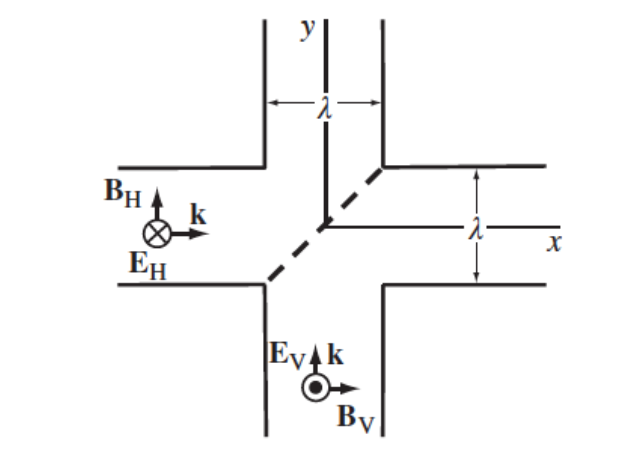
\includegraphics[width=6cm]{figures/crossbeams.png}
	\centering
	\caption{A sketch representation of the crossing beams and their components.}
\end{figure}

\textbf{a)}

The $\mathrm{H}$ and $\mathrm{V}$ beams are both propagating, monochromatic plane waves with electric field amplitude $E_{0}$. We know that the time-average density energy is given by:

\begin{equation}
	\langle u_{\mathrm{EM}} \rangle _{H, V}= \operatorname{Re}\left\{\frac{\epsilon_{0}}{4}\left(\mathbf{E} \cdot \mathbf{E}^{*}+c^{2} \mathbf{B} \cdot \mathbf{B}^{*}\right)\right\}=\frac{1}{2} \epsilon_{0} E_{0}^{2}.
\end{equation}

But at the very core of the intersection we are going to have a linear combination of $\mathbf{E}_{H}+\mathbf{E}_{V}$ and $\mathbf{B}_{H}+\mathbf{B}_{V}$, so this requires some computation to clean the following expression:
	
\begin{equation}
	\begin{split}
		\langle u_{\mathrm{EM}} \rangle_{\text{Total}}&= \operatorname{Re}\left\{\frac{\epsilon_{0}}{4}\left[\left(\mathbf{E}_{H}+\mathbf{E}_{V}\right) \cdot\left(\mathbf{E}_{H}^{*}+\mathbf{E}_{V}^{*}\right)+c^{2}\left(\mathbf{B}_{H}+\mathbf{B}_{H}\right) \cdot\left(\mathbf{B}_{H}^{*}+\mathbf{B}_{V}^{*}\right)\right]\right\}=\\
        &=\operatorname{Re}\left\{\frac{1}{4} \left( \epsilon_{0}\left(\mathbf{E}_{H}\mathbf{E}_{H}^{*} + \tfrac{1}{\epsilon_{0}\mu_{0}} \mathbf{B}_{H}\mathbf{B}_{H}^{*} \right)\right\}+\operatorname{Re}\left\{\frac{\epsilon_{0}}{4}\left(\mathbf{E}_{V}\mathbf{E}_{V}^{*} + \tfrac{1}{\epsilon_{0}\mu_{0}} \mathbf{B}_{V}\mathbf{B}_{V}^{*}\right) \right)\right\} +\\ 
		&\quad +\operatorname{Re}\left\{\frac{\epsilon_{0}}{4}\left(\mathbf{E}_{H}\mathbf{E}_{V}^{*} + \mathbf{E}_{V}\mathbf{E}_{H}^{*}+ \tfrac{1}{\epsilon_{0}\mu_{0}} \mathbf{B}_{H}\mathbf{B}_{V}^{*} +  \tfrac{1}{\epsilon_{0}\mu_{0}} \mathbf{B}_{V}\mathbf{B}_{H}^{*}\right)\right\}=\\
		&=\langle u_{\mathrm{EM}}\rangle_{H}+\langle u_{\mathrm{EM}}\rangle_{V}+\\
		&\quad+\operatorname{Re}\left\{\frac{\epsilon_{0}}{4}\left(\mathbf{E}_{H}\mathbf{E}_{V}^{*} + \mathbf{E}_{V}\mathbf{E}_{H}^{*}+ \tfrac{1}{\epsilon_{0}\mu_{0}} \mathbf{B}_{H}\mathbf{B}_{V}^{*} +  \tfrac{1}{\epsilon_{0}\mu_{0}} \mathbf{B}_{V}\mathbf{B}_{H}^{*}\right)\right\}. \\
	\end{split}
\end{equation}

Let us study some of the pieces of the last term in the previous line, so we can simplify even further. Observe that $\mathbf{B}_{H} \mathbf{B}_{V}^{*} = \mathbf{B}_{V} \mathbf{B}_{H}^{*} = 0$ because $\hat{y}\cdot \hat{x} = 0$. So the only possible contribution comes from:
	
\begin{equation}
	\mathbf{E}_{H} \mathbf{E}_{V}^{*} = - E_{0}^{2}\: e^{i(k x - ky)} \underbrace{\hat{z}\cdot\hat{z}}_{= 1}.
\end{equation}

And similarly for the other term with opposite sign in the exponent. So puting all together and recalling that $\left\langle u_{\mathrm{EM}}\right\rangle_{H, V}=\frac{1}{2} \epsilon_{0} E_{0}^{2}$, we have:
	
\begin{equation}
	\begin{split}
		\left\langle u_{\mathrm{EM}}\right\rangle_{Total}& =\tfrac{1}{2}\epsilon_{0} E_{0}^{2}+\tfrac{1}{2}\epsilon_{0} E_{0}^{2}-\tfrac{1}{2} \epsilon_{0} E_{0}^{2} \operatorname{Re}\underbrace{\left\{e^{i (k x - ky)} + e^{-i(kx- k y)}\right\}}_{=2 \cos(\arg)} =\\
		&=\tfrac{1}{2}\epsilon_{0} E_{0}^{2}\left[2- \cos (k\left[x-y\right])\right]
	\end{split}
\end{equation}

This quantity is minimum when $x=y$. On that plane (the diagonal of the crosswalk), the physical fields are:

\begin{equation}
	\mathbf{E}(x=y)=0 \hat{\mathbf{z}} \quad \text { and } \quad c \mathbf{B}(x=y)=E_{0} \cos (k x-\omega t)(\hat{\mathbf{x}}+\hat{\mathbf{y}})
\end{equation}

\textbf{b)}

Now we are asked to do exactly the same for the time-averaged Poynting vector for a plane wave propagating in the $\hat{\mathbf{k}}$ direction. This expression reads:

\begin{equation}
	\langle\mathbf{S}\rangle= \sqrt{\tfrac{\epsilon_{0}}{\mu_{0}}}|E_{0}|^{2}\hat{k}= c \left\langle u_{\mathrm{EM}}\right\rangle \hat{\mathbf{k}}.
\end{equation}

Therefore, the horizontal and vertical beams poynting expression follow from the previous part of the exercise as:

\begin{equation}
	\langle\mathbf{S}\rangle_{V}= c \epsilon_{0} E_{0}^{2} \hat{\mathbf{y}} \quad \text { and } \quad\langle\mathbf{S}\rangle_{H}= c \epsilon_{0} E_{0}^{2} \hat{\mathbf{x}}
\end{equation}

So the superposition reads:

\begin{equation}
	\begin{split}
		\langle\mathbf{S}\rangle &=\frac{1}{ \mu_{0}} \operatorname{Re}\left\{\left(\mathbf{E}_{H}+\mathbf{E}_{V}\right) \times\left(\mathbf{B}_{H}+\mathbf{B}_{V}\right)^{*}\right\}= \\
		&=\left\langle\mathbf{S}_{H}\right\rangle+\left\langle\mathbf{S}_{V}\right\rangle+\frac{1}{ \mu_{0}} \operatorname{Re}\left\{\mathbf{E}_{H} \times \mathbf{B}_{V}^{*}+\mathbf{E}_{V} \times \mathbf{B}_{H}^{*}\right\} =\\
		&= 2\: \epsilon_{0} \:c \: E_{0}^{2}(\hat{\mathbf{x}}+\hat{\mathbf{y}})-\frac{E_{0}^{2}  }{ \mu_{0}} \operatorname{Re}\underbrace{\left\{e^{i k(x-y)} \hat{\mathbf{y}}+e^{i k(y-x)} \hat{\mathbf{x}}\right\}}_{2\cos(\arg)} =\\
		&=2\:\epsilon_{0}\:c E_{0}^{2}[1- \cos k(x-y)](\hat{\mathbf{x}}+\hat{\mathbf{y}})
	\end{split}
\end{equation}

From this previous expression we can see that, again, something interesting will take place when $x=y$. Observe the following sketch. The Poynting vector grows outwards from the diagonal $x=y$.

\begin{figure}[h!]
	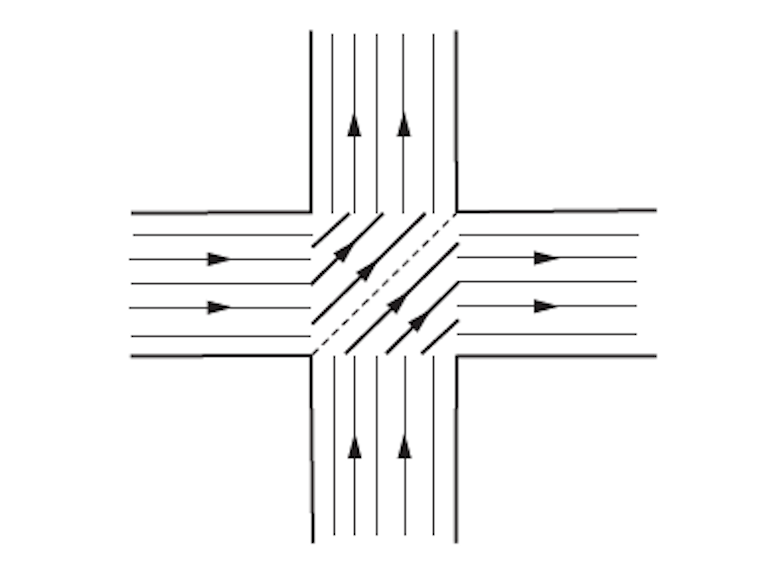
\includegraphics[width=6cm]{figures/electrocrosswalk.png}
	\centering
	\caption{The Poynting vector is nule in the $x=y$ diagonal.}
\end{figure}

\textbf{c)}

At the surface of a conductor, we must have $\mathbf{E}_{\|}=0$ and $\mathbf{B}_{\perp}=0$. For this problem, part (a) shows that $\mathbf{E}$ points along $\hat{\mathbf{z}}$ and goes to zero at $x=y .$ Part (a) showed also that $\mathrm{B}$ is parallel to the $x=y$ plane everywhere in the overlap region. Hence, the boundary conditions for a perfect conductor are met at $x=y$.




